\documentclass[tikz,border=8pt]{standalone}
\usepackage{amsmath}
\usetikzlibrary{arrows.meta,decorations.pathreplacing}
\begin{document}

% Asset ID: AS2DataPresentationTikZ-004
% Source: Histogram introduction evidence.
% Related lesson section: Core Theory, Histograms.
% Purpose: Show why unequal class widths require frequency density.
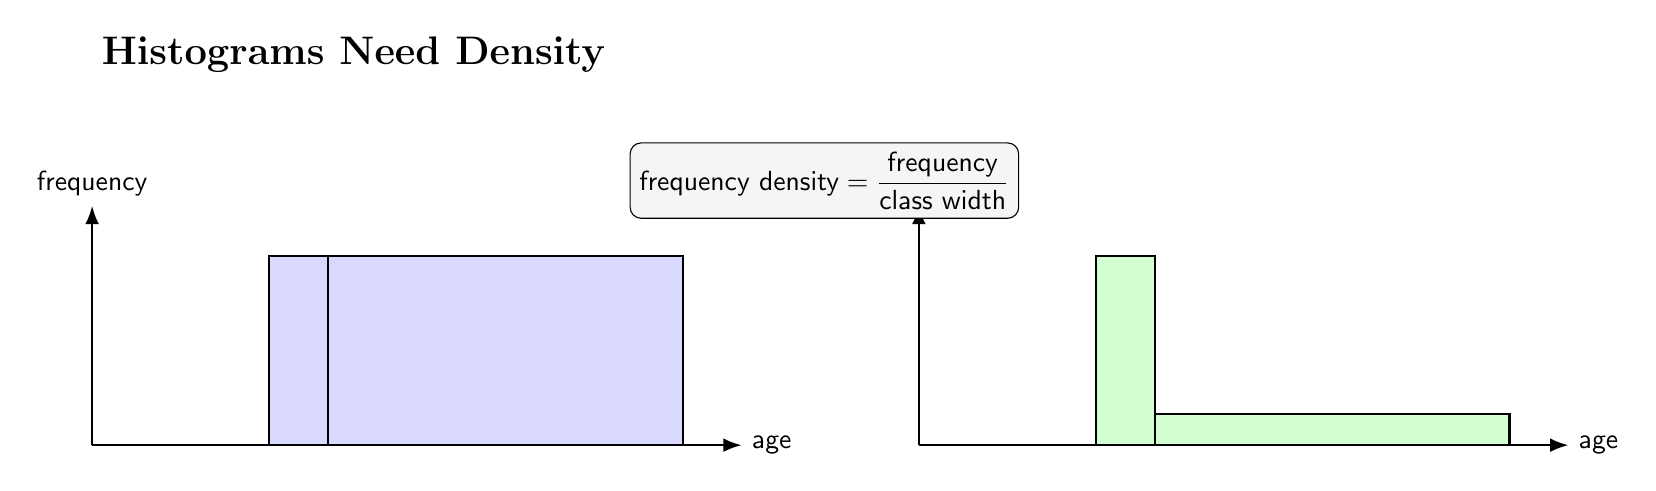
\begin{tikzpicture}[x=0.15cm,y=0.08cm,>=Latex,font=\sffamily]
\node[anchor=west,font=\bfseries\Large] at (0,62){Histograms Need Density};
\draw[->,thick] (0,0)--(55,0) node[right]{age}; \draw[->,thick] (0,0)--(0,38) node[above]{frequency};
\draw[fill=blue!15,thick] (15,0) rectangle (20,30); \draw[fill=blue!15,thick] (20,0) rectangle (50,30);
\begin{scope}[shift={(70,0)}]
\draw[->,thick] (0,0)--(55,0) node[right]{age}; \draw[->,thick] (0,0)--(0,38) node[above]{density};
\draw[fill=green!18,thick] (15,0) rectangle (20,30); \draw[fill=green!18,thick] (20,0) rectangle (50,5);
\end{scope}
\node[draw,rounded corners,fill=gray!8,align=center] at (62,42){$\text{frequency density}=\dfrac{\text{frequency}}{\text{class width}}$};
\end{tikzpicture}

\end{document}
